%% Separate medRxiv preprint built from the audited PeerJ manuscript.
\documentclass[10pt]{article}

\usepackage[letterpaper,margin=1in]{geometry}
\usepackage[T1]{fontenc}
\usepackage[utf8]{inputenc}
\usepackage[english]{babel}
\usepackage{mathptmx}
\usepackage{amsmath,amsfonts,amssymb,bm}
\usepackage{graphicx}
\usepackage{booktabs}
\usepackage{array}
\usepackage{tabularx}
\usepackage{textcomp}
\usepackage[round,authoryear]{natbib}
\usepackage{authblk}
\usepackage{caption}
\usepackage{lineno}
\usepackage{setspace}
\usepackage{ragged2e}
\usepackage{microtype}

%% Algorithm pseudocode
\usepackage[ruled,linesnumbered,vlined]{algorithm2e}
\usepackage[section]{placeins}
\usepackage{multirow}
\usepackage{needspace}

%% Preprint typography and paragraph layout.
\setlength{\parskip}{0.6em plus 0.1em minus 0.1em}
\setlength{\parindent}{0pt}
\setlength{\emergencystretch}{1em}
\setstretch{1.25}
\DeclareCaptionFont{singlespacing}{\setstretch{1}}
\captionsetup{font={small,singlespacing}}

%% Hyperlinks (load last)
\usepackage[colorlinks=true,linkcolor=black,citecolor=black,urlcolor=blue]{hyperref}

%% Custom shorthand
\newcommand{\dps}{$^{\circ}$/s}

\title{Criterion validity of heel-mounted inertial sensors for stride-length estimation during single- and dual-task walking in older adults with and without cognitive impairment}

\author[1]{Pawel Kudzia\thanks{Corresponding author: Pawel Kudzia, pawel.kudzia5@gmail.com}}
\author[1]{Markus von Hacht}
\author[1]{Maryam Sheikhi}
\author[1]{Drew Commandeur}
\author[1,2]{Marc Klimstra}
\author[1,3]{Sandra Hundza}
\affil[1]{Motion, Mobility and Rehabilitation Lab, School of Exercise Science, Physical and Health Education, University of Victoria, PO Box 1700 STN CSC, Victoria, BC V8W 2Y2, Canada}
\affil[2]{Canadian Sport Institute-Pacific, Victoria, BC, Canada}
\affil[3]{Institute on Aging and Lifelong Health, Victoria, BC}
\date{}

\newcommand{\preprintabstract}{%
\textbf{Background.} Gait metrics such as stride length are sensitive markers of fall and cognitive-decline risk in older adults, yet the reference systems that measure them accurately are limited to short walks in the laboratory. Wearable inertial sensors could extend monitoring into clinical and everyday settings, but their accuracy remains uncertain in the slow, variable gait of older adults.

\textbf{Methods.} We validated a heel-mounted inertial measurement unit (IMU) system against a GaitRite electronic walkway in 32 community-dwelling older adults (19 in the MoCA-defined cognitively normal group and 13 in the MoCA-defined cognitive impairment group). Participants completed single-task walking and three graded cognitive dual-task walking conditions (serial subtraction by 2s, 3s, and 7s) over a 6.1~m walkway. The pipeline combined bilateral stance detection with retroactive gravity-residual correction, used adaptive-threshold heel-strike and toe-off detection to support bilateral stance validation, and required no per-participant calibration.

\textbf{Results.} Across 10{,}472 matched strides retained after walk-level alignment quality control, stride length agreed with the walkway to within 3.9~cm root-mean-square error (RMSE), with a bias of $+0.3$~cm and an intraclass correlation (ICC) of 0.976. Mean absolute error fell below 4~cm in 31 of 32 participants. Per-condition RMSE ranged from 3.7 to 4.0~cm despite a 16\% drop in gait speed under the most demanding condition. Gait speed, stride time, and cadence also agreed closely with the walkway (ICC 0.90--0.96). Participant-level error was modestly higher in the MoCA-defined cognitive impairment group than in the cognitively normal group. Replacing the internal mid-stance integration anchor with GaitRite heel-strike timing did not reduce stride-length RMSE.

\textbf{Conclusions.} A calibration-free heel-mounted IMU pipeline maintained low stride-length error across graded dual-task walking in older adults. Error was low in both MoCA-defined groups. These findings establish criterion validity for successfully synchronised, supervised straight walkway passes and support further clinical evaluation. Everyday-living validity, other clinical cohorts, and test-retest reliability remain untested.
}

\begin{document}

\justifying
\raggedbottom
\pagenumbering{roman}

\begin{titlepage}
\maketitle
\thispagestyle{empty}
\vfill
\end{titlepage}

\pagenumbering{arabic}
\clearpage
\linenumbers
\section*{Abstract}
\preprintabstract

% ============================================================================
% INTRODUCTION
% ============================================================================

\clearpage
\section{Introduction}

\textbf{Gait metrics provide clinically relevant measures of mobility in older adults.}
Greater stride-to-stride variability is a strong predictor of incident falls in older adults \citep{Maki1997, Verghese2009}. Slower gait also predicts falls and cognitive decline \citep{Verghese2009, Montero-Odasso2012}. A meta-analysis reported that a baseline stride-length threshold of 0.64~m or less predicted adverse clinical events and mortality in older adults \citep{Bytyci2021}. Instrumented walkways and optical motion capture provide criterion measurements during short, controlled laboratory walks \citep{Webster2005, Arens2021}. Wearable inertial measurement units (IMUs) can extend stride-length measurement beyond these settings, but the quality of these estimates depends on both the measurement setup and the processing method.

\textbf{Sensor error, placement, and algorithm design all affect stride-length accuracy with foot-mounted IMUs.}
A common approach estimates stride length by integrating acceleration twice. Noise and small sensor errors accumulate during this process and cause the estimated position to drift \citep{Wahlstrom2020}. Sensor position and attachment influence the recorded signal and the resulting stride-length error \citep{Kuderle2022}. Zero-velocity updates (ZUPTs) limit drift by correcting the velocity estimate during stance, when the foot is stationary \citep{Foxlin2005, Wahlstrom2020}. These stationary anchors can bound each integrated stride. Adaptive thresholds can improve zero-velocity detection across walking speeds compared with a single fixed threshold \citep{Li2023}.

\textbf{Fixed amplitude thresholds can miss genuine stance phases and misclassify other stationary periods.}
During mid-stance the foot is still. Both the sensor's rotational speed (the gyroscope norm, the combined magnitude of triaxial angular velocity) and the moment-to-moment variation in its acceleration then drop close to zero. A threshold detector labels a sample as stance whenever both signals fall below fixed cutoffs \citep{Skog2010}. Fixed detector settings can fail when movement patterns differ from those used for tuning \citep{Foxlin2005}. Poor tuning can miss a true stance or label a non-walking stationary period as stance. A missed stance merges two adjacent integration intervals, while a false stance divides one interval.

\textbf{Bilateral ZUPT checks each candidate stance against movement of the opposite foot.}
During normal walking, one foot lifts from the ground shortly after the opposite foot enters stance. Arens et al. used contralateral toe-off information to identify an ipsilateral ZUPT during post-stroke walking \citep{Arens2021}. Our detector applies the same biomechanical relationship by accepting an ipsilateral stance candidate when contralateral toe-off falls within the expected time window. A recovery step also searches for quiet periods near unmatched opposite-foot toe-offs, allowing the detector to recover stances that a threshold alone missed. This check targets missed and false stance detections during variable gait.

\textbf{Two gaps remain in the evidence for this approach. The first is the lack of validation under cognitive load in older adults.}
One prior validation placed sensors on the foot and shank during straight, single-task walks in 10 healthy adults and 12 people with Parkinson's disease \citep{Sijobert2015}. Cognitive dual-task walking can slow gait and increase stride-to-stride variability \citep{Beauchet2005, Yogev-Seligmann2008, Hausdorff2008}. These changes broaden the range of gait speeds and patterns a pipeline must resolve and can make mid-stance harder to detect. The pipeline should be validated under these conditions rather than only during steady single-task walking. One heel-mounted IMU study assessed intra-session reliability in 101 middle-aged adults, including a cognitive dual-task condition, but did not validate against a criterion reference \citep{Boutaayamou2025}. Prior calibration-free validation included pathological cohorts walking at self-selected speed on an instrumented treadmill \citep{Laidig2021}. These protocols did not test graded cognitive load in older adults. Dual-task gait assessment has clinical relevance for evaluating fall risk and gait--cognition interactions \citep{Montero-Odasso2012, Commandeur2018, Springer2006}. To our knowledge, no prior study has validated gait-event detection and stride-length estimation against a criterion walkway in older adults under graded cognitive load across MoCA-defined cognitive status.

\textbf{The second gap concerns heel-mounted accuracy in older adults.}
A multi-position study in 14 healthy young adults found higher single-stride error at the heel than at five other foot-mounted locations, particularly during fast walking \citep{Kuderle2022}. Arens et al. used bilateral foot-mounted sensors and contralateral toe-off information in people post-stroke ($n = 8$), with optical motion capture as the reference \citep{Arens2021}. A heel-mounted bilateral ZUPT stance-detection and stride-length pipeline has not been validated against a criterion walkway in older adults walking under graded cognitive load.

\textbf{Our central contribution is validating two modifications to a calibration-free heel-mounted ZUPT pipeline under graded cognitive load.} We validated the pipeline against a GaitRite electronic walkway in 32 community-dwelling older adults. The cohort included 19 participants in the MoCA-defined cognitively normal group and 13 in the MoCA-defined cognitive impairment group. Participants walked under single-task and three graded cognitive dual-task conditions. The pipeline adds contralateral stance validation and retroactive gravity-residual correction to standard per-stride ZUPT integration. It requires no per-participant calibration. This design tests whether low stride-length error persists beyond steady single-task walking.

% ============================================================================
% METHODS
% ============================================================================

\clearpage
\section{Materials \& Methods}

\subsection{Participants}

\textbf{Thirty-two community-dwelling older adults completed the protocol after exclusions.}
We recruited 33 community-dwelling older adults aged 60 years or older, of whom 32 contributed to the analysis. The analysed cohort comprised 8 male and 24 female participants, with mean age $70.8 \pm 7.8$ years (range 60--83), mean height $167.4 \pm 7.6$~cm, and mean body mass $73.0 \pm 13.2$~kg (per-participant values in Supplementary Table~S1). Supplementary Table~S2 reports the two participant-condition records whose paired source data were unavailable. We formed two screening groups using the Montreal Cognitive Assessment (MoCA) \citep{Nasreddine2005}. The groups included 19 cognitively normal participants (CN, MoCA $\geq$ 26) and 13 participants meeting the MoCA criterion for cognitive impairment (CI, MoCA 14--25). These labels denote MoCA-defined screening groups rather than clinical diagnoses. Inclusion criteria were a MoCA score of 14 or higher and the ability to walk 20~m independently without a mobility aid. The University of Victoria Human Research Ethics Board approved the protocol (H22-00451), and all participants provided written informed consent.

\subsection{Instrumentation}

\textbf{Heel-mounted IMUs and a pressure-sensitive walkway provided the data analysed in this study.}
We attached two wireless IMUs (Opal, APDM Inc., Portland, OR) to the posterolateral heel of each shoe, adjacent to the calcaneus, using a 3D-printed housing fastened with a clip. We also placed an IMU over the sacrum for the broader study protocol, but we did not use its data in this analysis. Prior validation studies show the Opal sensor measures spatiotemporal gait parameters accurately against treadmill and instrumented-walkway references in healthy adults and older adults \citep{Washabaugh2017, Morris2019}. Each heel IMU recorded triaxial accelerometer ($\pm$16~g) and gyroscope ($\pm$2000\dps) data at 256~Hz.

A pressure-sensitive electronic walkway (GaitRite, model Platinum, CIR Systems Inc., Franklin, NJ) served as the criterion reference. The walkway has an active sensing area of 594~cm $\times$ 61~cm with 1.27~cm square sensors that record heel-on to toe-off stance events for each foot at 120~Hz. GaitRite gait parameters show excellent concurrent validity against three-dimensional motion capture, with ICC 0.92--0.99 across walking speed, cadence, step length, and step time \citep{Webster2005}. We synchronised the walkway and IMU clocks using a GaitRite Pulse (GR Pulse) signal generated by a custom-written LabVIEW program. The GR Pulse marked the start and end of each walkway pass on the LabVIEW clock. Within each participant-condition pair, we fitted a linear clock correction between GR Pulse rising edges and corresponding IMU activity onsets across up to seven walks. We then estimated a residual constant offset within each walk by aligning adaptive-detector IMU heel strikes with GaitRite heel strikes.

\subsection{Protocol}

\textbf{Each participant completed four walking conditions, one single-task and three graded dual-task conditions.}
Single-task walking served as the baseline, followed by three dual-task conditions of graded cognitive difficulty. Participants counted backwards aloud by 2s, 3s, and 7s from a random three-digit starting number while walking. Each condition comprised seven trials of two passes (out and back) over the GaitRite mat at a self-selected comfortable pace. This yielded 14 walks per condition and 56 walks per participant across the four reported conditions. Participants walked beyond both ends of the mat to allow acceleration and deceleration off the recording surface. Participants wore a safety belt, and a spotter accompanied them. We provided rest periods between conditions as needed.

\subsection{Signal preprocessing}

\textbf{We bandpass-filtered the gyroscope signal and aligned the left-right sign convention before further processing.}
We first bandpass-filtered raw gyroscope signals (0.5--10~Hz, fourth-order Butterworth) to remove low-frequency drift and high-frequency noise. We then inverted the left heel gyroscope Z-axis to match the right heel sign convention (positive = plantarflexion angular velocity in the sagittal plane). We left the triaxial accelerometer signals unfiltered for the ZUPT integration pipeline. The per-stride zero-velocity and gravity-residual corrections addressed integration drift directly, so we did not add an accelerometer filter whose cutoff would require further tuning.

\begin{figure*}[!ht]
\centering
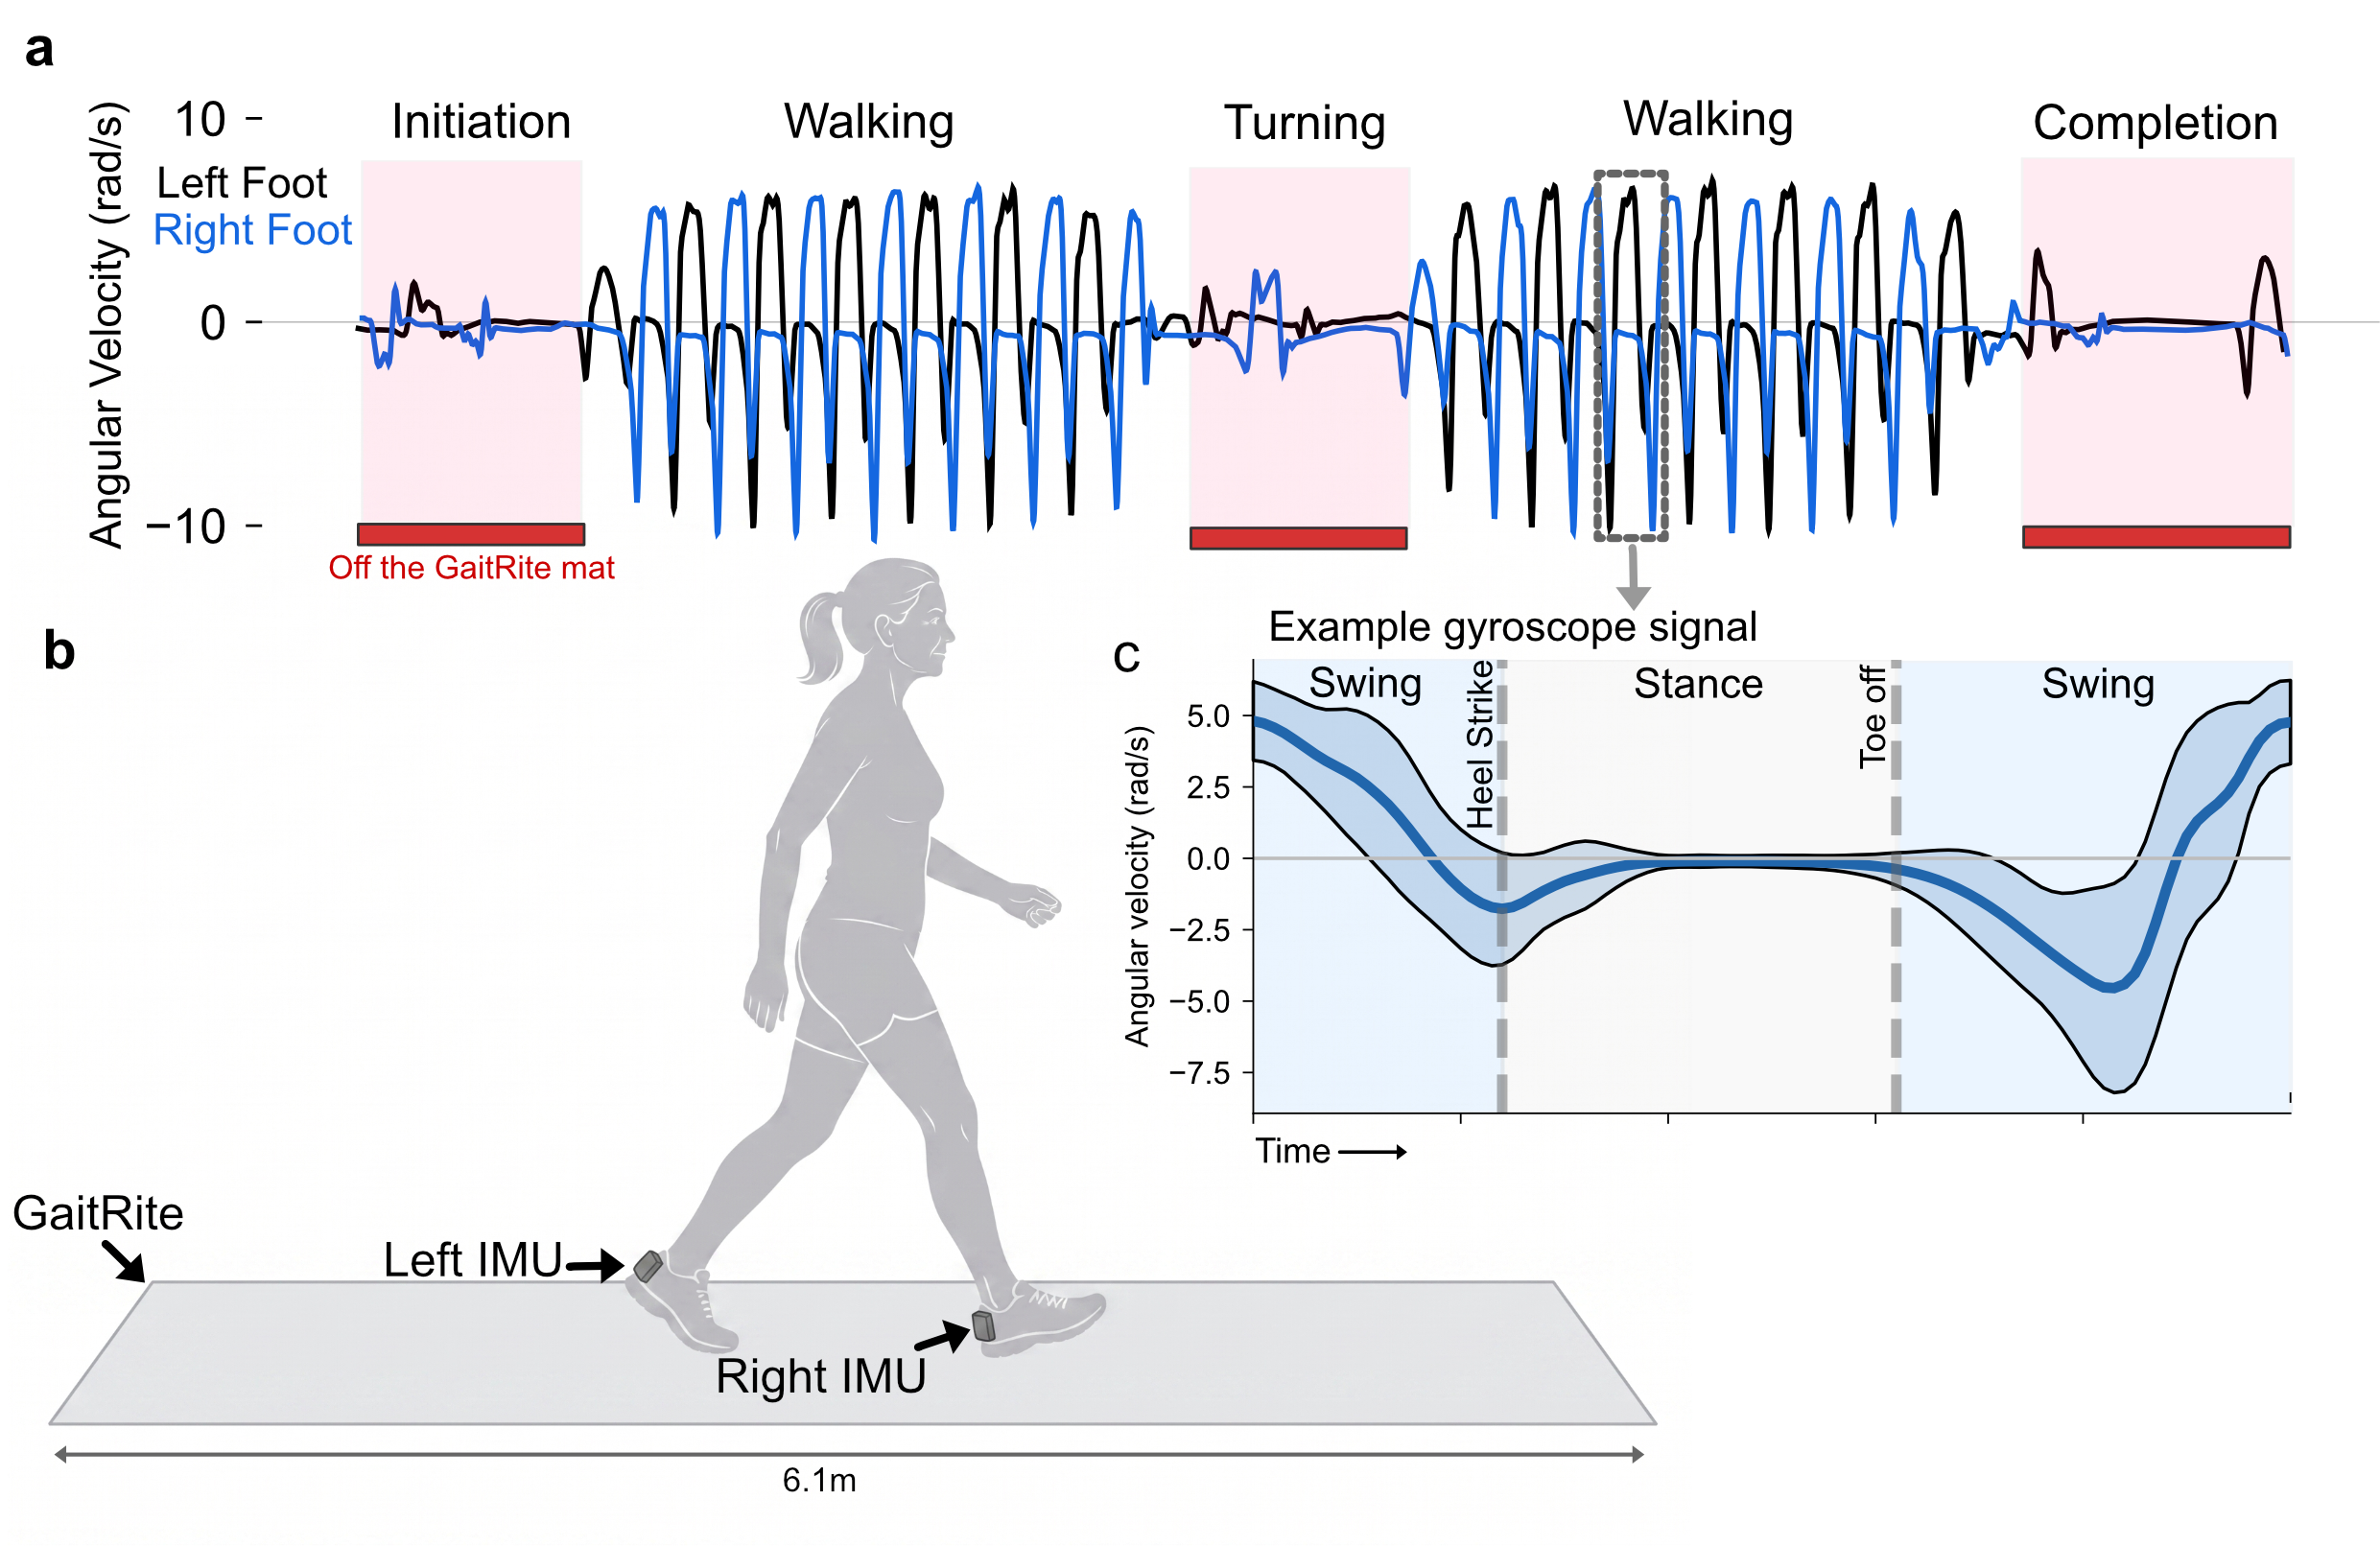
\includegraphics[width=\textwidth]{figures/Figure1.png}
\caption{Experimental setup and gyroscope processing.
(a) Filtered sagittal-plane signals from the left (black) and right (blue) heel IMUs during one out-and-back trial. Labels mark activity phases, red bars mark off-mat intervals, and the highlighted box is expanded in panel~c.
(b) Sensor placement during GaitRite walking. Heel IMUs were clipped to the posterolateral aspect of each shoe using 3D-printed housings. A sacrum-mounted IMU was present as part of the broader protocol, but its data were not used in this analysis.
(c) Mean right-heel gyroscope Z-axis signal over a normalized gait cycle, pooled across participants and conditions. The Z-axis captures sagittal-plane angular velocity. The blue line shows the mean, shading shows $\pm 1$~SD, dashed lines mark heel strike and toe off, and labels identify swing and stance.}
\label{fig:methods}
\end{figure*}

\needspace{4\baselineskip}
\subsection{Gait event detection}\label{sec:events}

\textbf{We detected heel strikes and toe-offs on each foot using thresholds that adapted to the participant's walking pattern.} A fixed cutoff can miss events when stride amplitudes change with walking pace. We therefore adapted an established sagittal-plane gyroscope detector \citep{Salarian2004} using signal-derived thresholds \citep{Greene2010}. The detector estimated stride frequency from the repeating pattern of the filtered gyroscope signal. Heel-strike and toe-off peak thresholds used 35\% and 30\% of the negative-peak amplitude interquartile range, respectively. Cadence scaled both thresholds. The peak threshold could not fall below 15\% of the maximum absolute signal amplitude or 0.5~rad/s. Positive swing confirmation used 25\% of the maximum absolute amplitude with a 1.0~rad/s floor. The detector then classified negative signal peaks according to the pattern that followed within 80--220~ms. A rapid rise into swing identified toe-off, while a near-zero segment identified heel strike (Fig.~\ref{fig:methods}c). Toe-offs supported bilateral stance validation, and both events were compared with GaitRite for the timing analysis. Stride time for paired analyses came from consecutive stance midpoints because these stationary anchors also bounded each integrated displacement. We analysed discrete heel-strike timing separately against GaitRite initial contacts.

\subsection{Ipsilateral stance phase detection with contralateral validation}\label{sec:stance}

\textbf{Stance-phase detection runs in two steps.} A low-motion detector first finds candidate stance windows on one foot. A toe-off on the opposite foot then confirms each candidate. Here, ipsilateral means the foot being evaluated and contralateral means the opposite foot. The resulting stance mask anchors the ZUPT integration. We define stride boundaries at the midpoints of consecutive stance phases because the foot is stationary there, providing a stable zero-velocity reference.

\textit{Step 1. Ipsilateral low-motion detection.} The detector evaluated gyroscope magnitude and accelerometer variability from the same heel sensor, following established fixed-threshold approaches \citep{Skog2010, Foxlin2005}. We used a sliding 40~ms window. A sample qualified as a stance candidate when both signals fell below adaptive thresholds calculated for each participant and walking condition. The gyroscope criterion identified low rotation during foot-flat contact, while the accelerometer criterion rejected brief low-rotation periods during swing. Algorithm~\ref{alg:bilateral_zupt} lists the thresholds, limits, and recovery window used in the analysis.

\textit{Step 2. Opposite-foot confirmation.} The detector used opposite-foot toe-off information to confirm stance candidates, following the bilateral approach of \citet{Arens2021}. We accepted a candidate when an opposite-foot toe-off fell within 150~ms of either boundary of the candidate segment. Candidates without a matching toe-off were rejected. An unmatched toe-off triggered a recovery search for a quiet period on the other foot. The detector also removed very short stance segments, joined segments separated by brief gaps, and checked unusually long strides for a missed stance. These steps reduced false detections during stops and prevented two strides from being merged.

\textit{Fallback to threshold-only detection.} The pipeline reverts to ipsilateral threshold-only stance detection whenever contralateral validation returns an implausibly low stance count. We defined this as fewer than three validated segments or fewer than 50\% of the threshold-only segments when the threshold-only detector found at least ten. This guard fired in 11 of 256 subject-condition-foot units (4.3\%). Eight of the 11 units came from a single participant whose contralateral toe-off detection failed in every condition. Most paired strides therefore used contralateral validation, while the fallback prevented loss of otherwise usable data when contralateral event detection failed.

\subsection{ZUPT stride length integration}

\textbf{We estimated stride length by double-integrating the accelerometer signal between consecutive stance midpoints.} During each stance phase the foot rests on the ground at zero velocity. The stance mask from Section~\ref{sec:stance} flags these zero-velocity intervals, which are used to correct the drift that double integration would otherwise produce \citep{Foxlin2005, Skog2010}. We estimated gyroscope and accelerometer biases once per walking bout, defined as a run of consecutive stance phases separated by no gap longer than 3~s. The stance phase supplies the reference, because true angular rate is zero and true acceleration equals gravity. We bias-corrected the signals with these estimates before integration, removing the slow sensor offsets that would otherwise accumulate as drift.

\subsubsection{Orientation tracking}

\textbf{We tracked sensor orientation with a Mahony attitude-and-heading reference system.} This filter combines gyroscope and accelerometer measurements to estimate how the sensor is oriented relative to gravity \citep{Mahony2008}. We used a higher correction gain during stance ($K_p = 1.0$), when the stationary foot provides a reliable gravity reference, and a lower gain during swing ($K_p = 0.05$), when movement affects the accelerometer signal. The integral gain remained at $K_i = 0.02$. We reduced the proportional accelerometer correction gain during swing to limit contamination by dynamic acceleration. This follows the movement-gating rationale of foot-mounted filters that disable accelerometer-based orientation updates during swing \citep{Hannink2017}.

\subsubsection{Gravity removal, double integration, and stride length extraction}

\textbf{We integrated the gravity-removed acceleration twice between consecutive stance midpoints to estimate stride length.} We rotated the bias-corrected accelerometer signal into the navigation frame using the Mahony-estimated orientation, subtracted gravity, and double-integrated to obtain velocity and position \citep{Foxlin2005}. Because the foot is momentarily stationary at each stance boundary, its true velocity is zero. We applied a linear zero-velocity correction that distributes the accumulated velocity error backward across the preceding swing samples and then resets the velocity to that known zero, cancelling the drift built up over the stride. Each stride integrates independently with position and velocity reset at each stance midpoint, which bounds drift to a single swing phase. Stride length is the magnitude of the horizontal component of the 3D displacement between consecutive stance midpoints. We accepted strides with duration 0.4--2.0~s, length 0.3--2.5~m, and minimum gyroscope amplitude 3.0~rad/s, a low floor that excludes near-stationary segments rather than genuine strides.

\subsubsection{Retroactive gravity-residual correction}

\textbf{We corrected the acceleration residual that remained after orientation tracking and gravity removal.} The code refers to this step as bidirectional smoothing. Small orientation errors during swing leave a horizontal acceleration residual after gravity removal, which can bias the integrated stride length \citep{Foxlin2005, Hannink2017}. The correction reduced this positive offset in the current cohort (Supplementary Table~S4).

We corrected this residual retroactively after each swing phase. At each stance onset we measured the residual. We skipped the first 10~ms to avoid the heel-strike impact transient, then averaged the navigation-frame acceleration over the next 20~ms. We then subtracted a linear ramp of this residual through the preceding swing samples, scaled by a gain of 0.5:
\begin{equation}
\mathbf{a}_{\text{corrected}}(t) = \mathbf{a}_{\text{nav}}(t) - 0.5 \cdot \frac{t}{T_{\text{swing}}} \cdot \mathbf{r}
\end{equation}
where $t$ is time from swing onset, $T_{\text{swing}}$ is swing duration, and $\mathbf{r}$ is the gravity residual at the next stance onset. We selected the gain of 0.5 empirically in this cohort because no prior work specifies a value for this correction. This selection was not independent of the validation sample. The correction operates per stride and requires no external calibration. A sensitivity analysis across gains from 0.3 to 0.7 showed pooled RMSE values from 3.83 to 4.10~cm (Supplementary Table~S7).

\subsubsection{Algorithm summary}

\textbf{Algorithm~\ref{alg:bilateral_zupt} summarises the complete processing sequence.} Step~1 builds the stance mask using low-motion detection and opposite-foot confirmation. Step~2 tracks orientation, removes gravity, integrates each stride, and applies the retroactive gravity-residual correction before resetting velocity. Contralateral stance validation and the gravity-residual correction distinguish the tested pipeline from a standard ZUPT implementation \citep{Foxlin2005, Skog2010}.

\begin{algorithm}[!ht]
\SetAlgoLined
\DontPrintSemicolon
\SetKwInOut{Input}{Input}
\SetKwInOut{Output}{Output}
\Input{Ipsilateral 3-axis accelerometer (\texttt{accel}) and gyroscope (\texttt{gyro})\\
       Contralateral toe-off times (\texttt{contra\_to})\\
       Sampling rate (\texttt{fs})}
\Output{Stride lengths (\texttt{stride\_lengths})}
\tcc{Step 1. Stance detection with contralateral validation}
\texttt{gyro\_norm}     $=$ magnitude of \texttt{gyro} at each sample\;
\texttt{accel\_var}     $=$ 40 ms sliding variance of \texttt{accel}\;
\texttt{gyro\_thresh}   $=$ clip(15th percentile of \texttt{gyro\_norm},\; 0.3, 2.0 rad/s)\;
\texttt{accel\_thresh}  $=$ clip(25th percentile of \texttt{accel\_var},\; 0.2, 5.0 (m/s$^2$)$^2$)\;
\texttt{candidates}     $=$ samples where \texttt{gyro\_norm} $<$ \texttt{gyro\_thresh} \textbf{and} \texttt{accel\_var} $<$ \texttt{accel\_thresh}\;
\For{each candidate segment}{
  \eIf{any \texttt{contra\_to} event falls within $\pm$150 ms of the segment boundary}{
    accept segment as stance\;
  }{
    reject segment\;
  }
}
recover missed stances near unmatched \texttt{contra\_to} using relaxed gyroscope-only threshold (25th percentile, 0.5 rad/s floor)\;
reject stance segments $<$ 30 ms, merge segments separated by $<$ 75 ms, split strides $>$ 1.8 s at a mid-stride quiet period\;
\tcc{Step 2. Per-stride integration with retroactive gravity-residual correction}
estimate \texttt{gyro\_bias} and \texttt{accel\_bias} from stance samples of each walking bout\;
\For{each stride between consecutive stance midpoints}{
  track orientation with Mahony AHRS (gain 1.0 during stance, 0.05 during swing)\;
  rotate (\texttt{accel} $-$ \texttt{accel\_bias}) into the navigation frame, subtract gravity\;
  measure gravity residual at the next stance onset\;
  subtract a linear ramp of that residual through the preceding swing (gain 0.5)\;
  integrate corrected acceleration $\rightarrow$ \texttt{velocity}, distribute the accumulated velocity error linearly back across the swing, then set \texttt{velocity}=0 at stance ends\;
  integrate \texttt{velocity} $\rightarrow$ \texttt{position}\;
  \texttt{stride\_length} $=$ horizontal distance between stride start and stride end positions\;
  reject stride unless duration 0.4--2.0 s, length 0.3--2.5 m, peak \texttt{gyro\_norm} $>$ 3.0 rad/s\;
}
\Return \texttt{stride\_lengths}\;
\caption{Bilateral ZUPT stride-length estimation.}
\label{alg:bilateral_zupt}
\end{algorithm}

\subsection{GaitRite stride matching}\label{sec:matching}

\textbf{We paired each ZUPT stride with its GaitRite counterpart using clock alignment and stride-level checks.} The GR Pulse correction placed each walk on the IMU timeline, and heel-strike alignment supplied a final offset within each walk. We accepted a walk-level alignment only when at least 60\% of the expected GaitRite heel strikes had an IMU match within 150~ms. This required most reference events to match while allowing one or two missed detections in a short pass. Walks without a valid alignment were classified as synchronisation failures and did not enter paired stride or event-agreement analyses. We paired strides from the same foot when the IMU and GaitRite stride midpoints were each other's closest match. The allowable time difference adapted to stride duration and never exceeded 0.5~s. We retained GaitRite strides with lengths of 0.30--2.00~m and times of 0.40--1.80~s. The matched IMU length and time also had to fall between 50\% and 150\% of the corresponding reference value. We call this the stride-pair mismatch filter. It removed likely pairing errors and GaitRite records in which a missed heel strike produced an apparent double stride.

We retained only strides that fell completely within a GaitRite walk window. This removed turns, off-mat acceleration and deceleration, mat-entry transitions, and rest periods. Participants began walking approximately 1~m before the mat, so gait-initiation strides were not part of the synchronised comparison. Partial steps at either end of the mat were removed before matching.

\textbf{The final analysis included 10{,}472 paired strides from 32 participants.} We excluded one of the 33 enrolled participants because the required heel-mounted IMU recordings were unavailable. We retained every reported participant-condition record that had the required source data and at least one stride pair after the common matching rules. We did not exclude records based on match count or stride-length error because both are study outcomes. GR Pulse records were unavailable for ID\_186 L2 and ID\_195 L2, so these two conditions could not enter the paired analysis (Supplementary Table~S2). Of 1{,}764 available walks, 1{,}669 passed alignment QC and 95 were classified as synchronisation failures. Failures occurred in 14 single-task, 13 serial-2, 19 serial-3, and 49 serial-7 walks. We also excluded three individual walks for documented data-quality problems described in Supplementary Section~S2. After stride-level checks, the final pool contained 2{,}544 single-task, 2{,}618 serial-2, 2{,}770 serial-3, and 2{,}540 serial-7 strides. The conditions included 32, 30, 32, and 32 participants, respectively.

\subsection{Outcome measures and statistical analysis}\label{sec:outcomes}

\textbf{The primary outcome was pooled stride-level RMSE between IMU and GaitRite stride length.} Agreement outcomes included signed bias, SD of the error, 95\% limits of agreement, MAE, ICC(2,1), and proportional bias. We calculated bias and limits of agreement following \citet{Bland1986} and ICC(2,1) following \citet{Shrout1979}. We also reported the percentage of strides within 5 and 10~cm and calculated RMSE and MAE at the participant level. Event-detection outcomes were miss rate, timing bias, and RMSE against GaitRite heel strikes and toe-offs. A missed event had no IMU match within 150~ms. To assess stride-to-stride consistency, we calculated stride-length coefficient of variation for each participant and condition and compared the IMU and GaitRite values using bias, RMSE, and ICC(2,1).

We evaluated gait parameters other than stride length using RMSE, bias, and ICC(2,1). We also performed two design comparisons. First, we ran the full stride-length pipeline with bilateral and ipsilateral threshold-only stance detection while keeping all other parameters identical. We compared matched stride pairs, RMSE, bias, and ICC between methods. Second, we compared the internal mid-stance integration boundaries with GaitRite-derived heel-strike boundaries. For this comparison, we used RMSE, bias, MAE, SD of the error, 95\% limits of agreement, and ICC(2,1).

We tested the effect of cognitive load on stride-length accuracy with a repeated-measures analysis of variance (ANOVA) on participant-level mean absolute error, restricted to the 30 participants with valid data in all four conditions. We applied the Greenhouse--Geisser correction when Mauchly's test indicated a sphericity violation. We then ran pairwise condition comparisons with Bonferroni correction and focused reporting on each dual-task condition against single-task walking. We report generalised eta-squared ($\eta^2_G$) for the overall ANOVA. We compared participant-level MAE between the MoCA-defined groups with a two-sided Mann--Whitney test. This subgroup analysis was exploratory and was not adjusted for multiple comparisons. We described the stride-level relationship between gait speed and absolute error using linear regression and reported $R^2$ without using the regression for participant-level inference. Participant MAE confidence intervals in Fig.~\ref{fig:subject_accuracy} used 2{,}000 walk-cluster resamples. We ran all analyses in Python 3.13 with pingouin 0.6.1, statsmodels 0.14.6, and scipy 1.17. We selected and reported reliability and agreement measures following the Guidelines for Reporting Reliability and Agreement Studies (GRRAS) \citep{Kottner2011}.

\textbf{We assessed cohort-level accuracy with a participant-clustered bootstrap.} We resampled the 32 participants with replacement and recomputed RMSE, MAE, bias, and ICC on the resulting stride pool. We repeated this process 10{,}000 times to obtain 95\% percentile confidence intervals. The sample size was based on participant availability rather than a prospective power calculation.

\textbf{We ran two sensitivity analyses.} First, we repeated the accuracy analysis without the stride-pair mismatch filter defined above. All other matching and filtering rules remained unchanged. This analysis tested whether the filter affected the reported accuracy. Second, we varied the retroactive gravity-residual correction gain from 0.3 to 0.7 in increments of 0.1 while keeping the rest of the pipeline unchanged. We compared retained pairs, RMSE, MAE, bias, and ICC(2,1). These same-cohort analyses assess robustness to analysis choices but do not replace independent validation.

% ============================================================================
% RESULTS
% ============================================================================

\clearpage
\section{Results}

\FloatBarrier
\subsection{Gait event detection accuracy}

\textbf{The adaptive-threshold detector matched GaitRite heel strikes within 33~ms RMSE and toe-offs within 39~ms RMSE.}
Heel-strike miss rates ranged from 0.0\% to 0.4\% and toe-off miss rates from 2.8\% to 3.8\% across conditions (Table~\ref{tab:events}). Heel-strike RMSE was 27--33~ms and toe-off RMSE was 33--39~ms. A missed event denotes a heel strike or toe-off that the detector could not localise within a stride the pipeline had identified.

\begin{table*}[!ht]
\centering
\caption{Adaptive-threshold gait-event accuracy. HS = heel strike; TO = toe off. Miss rate is the percentage of GaitRite events unmatched within 150~ms. Bias = mean IMU-minus-GaitRite timing error.}
\label{tab:events}
\small
\begin{tabular}{@{}llrrrrr@{}}
\toprule
Condition & Event & Miss rate (\%) & $N$ matched & Bias (ms) & RMSE (ms) & MAE (ms) \\
\midrule
Single-task & HS & 0.0 & 3749 & $-0.7$ & 26.8 & 16.7 \\
            & TO & 2.8 & 3698 & +3.9 & 32.8 & 22.7 \\
Serial 2s   & HS & 0.2 & 3650 & $-0.2$ & 31.2 & 18.8 \\
            & TO & 3.2 & 3586 & $-0.7$ & 37.8 & 25.9 \\
Serial 3s   & HS & 0.4 & 3858 & +0.1 & 32.4 & 19.8 \\
            & TO & 3.6 & 3760 & 0.0 & 38.7 & 26.6 \\
Serial 7s   & HS & 0.4 & 3554 & +0.1 & 32.6 & 20.1 \\
            & TO & 3.8 & 3499 & +1.7 & 39.3 & 27.3 \\
\bottomrule
\end{tabular}
\end{table*}

\FloatBarrier
\subsection{Stance detection and event-timing comparisons}

\textbf{Bilateral validation recovered more reference strides with similar accuracy.} On the GaitRite-labelled strides, bilateral validation recovered 10{,}472 matched pairs compared with 9{,}708 for threshold-only detection (Table~\ref{tab:design}). The two methods differed by 0.1~cm RMSE and both returned an ICC of 0.976.

\textbf{Substituting GaitRite heel-strike timing for the internal mid-stance anchor did not reduce stride-length error.} We re-ran the ZUPT integrator with GaitRite-derived heel-strike times as displacement endpoints on the 10{,}459 strides matched in both anchoring schemes. RMSE rose from 3.9 to 4.1~cm and ICC fell from 0.976 to 0.973 (Table~\ref{tab:design}).

\begin{table*}[!ht]
\centering
\caption{Pipeline design comparisons. The blocks compare stance detection and integration anchors on their respective shared stride sets, so $N$ differs. All other pipeline steps were held constant. Bias = IMU minus GaitRite.}
\label{tab:design}
\small
\begin{tabular}{@{}lrrrrc@{}}
\toprule
Variant & $N$ pairs & RMSE (cm) & Bias (cm) & MAE (cm) & ICC(2,1) \\
\midrule
\multicolumn{6}{@{}l}{\textit{Stance detection}} \\
Bilateral (canonical)        & 10,472 & 3.9 & $+0.3$ & 2.5 & 0.976 \\
Ipsilateral (threshold-only) & 9,708 & 3.8 & $-0.3$ & 2.4 & 0.976 \\
\midrule
\multicolumn{6}{@{}l}{\textit{Gait-event timing anchor}} \\
Mid-stance (canonical)       & 10,459 & 3.9 & $+0.3$ & 2.5 & 0.976 \\
GaitRite heel strike         & 10,459 & 4.1 & $+1.1$ & 2.8 & 0.973 \\
\bottomrule
\end{tabular}
\end{table*}

\FloatBarrier
\subsection{Stride length accuracy}\label{sec:results_accuracy}

\textbf{The pipeline measured stride length with 3.9~cm RMSE and 2.5~cm MAE.} The pooled analysis included 10{,}472 matched stride pairs and returned an ICC of 0.976. Bias was $+0.3$~cm and the SD of error was 3.9~cm (Table~\ref{tab:accuracy}, Fig.~\ref{fig:scatter}). The scatter plot shows agreement across the full stride-length range (Fig.~\ref{fig:scatter}a). The Bland-Altman plot shows a small mean bias and a weak trend across the range (Fig.~\ref{fig:scatter}b; proportional-bias slope 0.036). Per-condition RMSE ranged from 3.7 to 4.0~cm, and per-condition ICC ranged from 0.971 to 0.977. The conditions included 32, 30, 32, and 32 participants (Table~\ref{tab:accuracy}). The error fell within $\pm 5$~cm for 87\% of stride pairs and within $\pm 10$~cm for 97\%. Proportional bias was weak (slope $0.036$, $R^2 = 0.026$). Relative to the mean GaitRite stride length of 1.20~m, pooled RMSE was 3.2\% and MAE was 2.1\%.

Bias was positive across all four conditions and error distributions overlapped (Table~\ref{tab:accuracy}). Participant-level MAE ranged from 1.6 to 4.7~cm, with 31 of 32 participants below 4~cm (Fig.~\ref{fig:subject_accuracy}). Mean per-participant RMSE was 3.8~cm and ranged from 2.1 to 7.2~cm.

When we disabled the retroactive gravity-residual correction on the same matched strides, pooled RMSE and bias increased (Supplementary Table~S4).

\begin{table*}[!ht]
\centering
\caption{Bilateral ZUPT stride-length accuracy by condition. $n$ = participants; $N$ = matched stride pairs; bias = mean IMU-minus-GaitRite error; LoA = Bland--Altman 95\% limits of agreement.}
\label{tab:accuracy}
\small
\begin{tabular}{@{}lrrrrrrr@{}}
\toprule
Condition & $n$ & $N$ pairs & Bias (m) & RMSE (m) & MAE (m) & 95\% LoA (m) & ICC(2,1) \\
\midrule
Single-task & 32 & 2,544 & +0.007 & 0.040 & 0.027 & [$-0.069$, +0.084] & 0.973 \\
Serial 2s   & 30 & 2,618 & +0.001 & 0.037 & 0.024 & [$-0.072$, +0.073] & 0.977 \\
Serial 3s   & 32 & 2,770 & +0.000 & 0.039 & 0.024 & [$-0.077$, +0.077] & 0.975 \\
Serial 7s   & 32 & 2,540 & +0.003 & 0.039 & 0.025 & [$-0.073$, +0.078] & 0.971 \\
\midrule
Pooled      & 32 & 10,472 & +0.003 & 0.039 & 0.025 & [$-0.073$, +0.078] & 0.976 \\
\bottomrule
\end{tabular}
\end{table*}

\begin{figure*}[!ht]
\centering
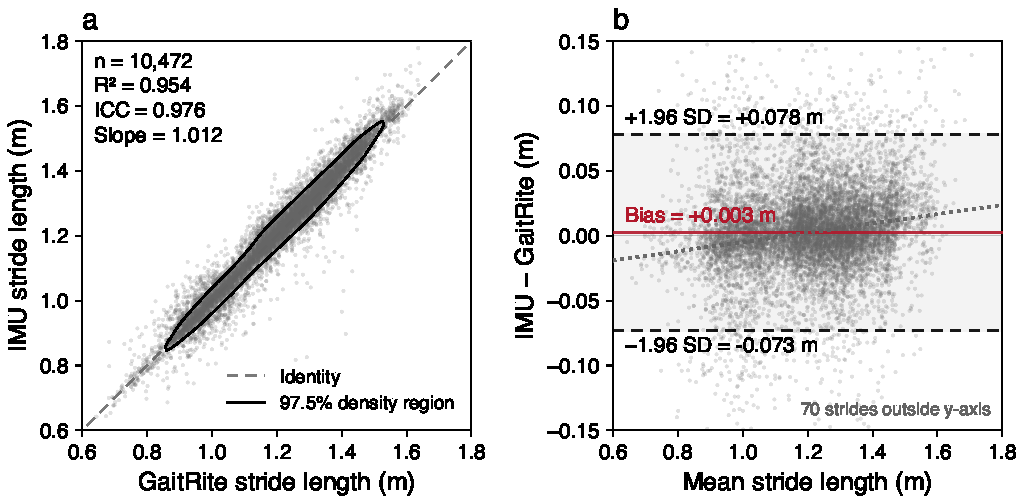
\includegraphics[width=\textwidth]{figures/Figure2.pdf}
\caption{Stride length agreement between IMU and GaitRite.
(a) All 10{,}472 matched strides. The dashed line marks identity, and the contour encloses the densest 97.5\% of points. Linear fit $R^2 = 0.954$, slope = 1.012, and ICC(2,1) = 0.976.
(b) Bland--Altman plot. The red line marks mean bias ($+0.003$~m), dashed lines mark the 95\% limits of agreement ($-0.073$ to $+0.078$~m), and the dotted line shows proportional bias (slope = 0.036).}
\label{fig:scatter}
\end{figure*}

\begin{figure*}[!ht]
\centering
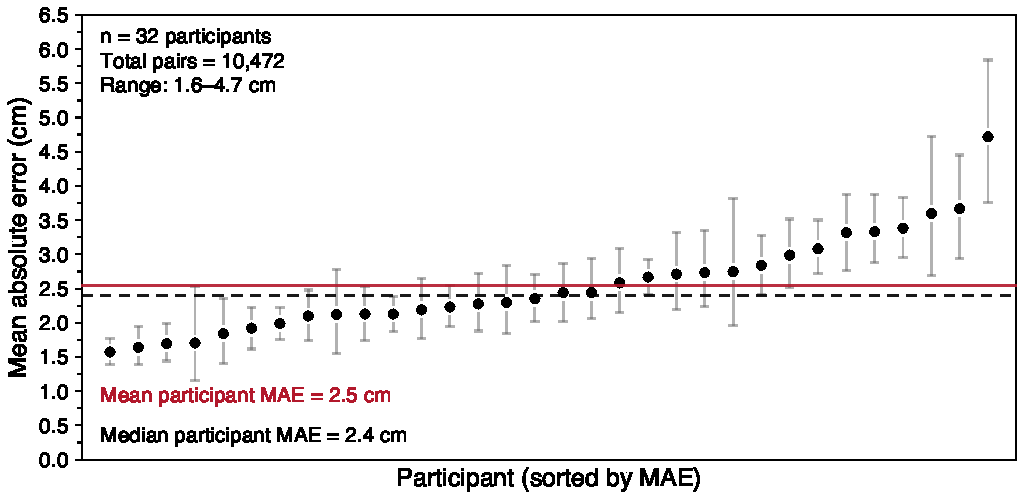
\includegraphics[width=\textwidth]{figures/Figure3.pdf}
\caption{Participant stride-length accuracy across conditions ($n = 32$). Dots show participants sorted by MAE with 95\% CIs. The solid red and dashed grey lines mark the mean (2.5~cm) and median (2.4~cm), respectively.}
\label{fig:subject_accuracy}
\end{figure*}

\FloatBarrier
\subsubsection{Effect of cognitive load and cognitive status on stride length accuracy}

\textbf{Accuracy did not differ across walking conditions, but participant-level error was modestly higher in the MoCA-defined CI group.}
The repeated-measures ANOVA on participant-level MAE included the 30 participants with data in all four conditions. It found no evidence of a condition effect ($F(2.35, 68.27) = 0.67$, Greenhouse--Geisser corrected $p$ = .541, $\eta^2_G = 0.016$). No comparison between single-task and a dual-task condition was significant after Bonferroni correction. Absolute error was also weakly related to gait speed ($R^2 = 0.002$). Mean signed bias was below 1~cm in every condition (Table~\ref{tab:accuracy}).

Stratified by MoCA-defined cognitive status, RMSE was 3.65~cm in CN participants ($n = 19$, 6{,}139 strides) and 4.14~cm in CI participants ($n = 13$, 4{,}333 strides). Median per-participant MAE was 2.28~cm in the CN group and 2.84~cm in the CI group (Mann--Whitney $U = 71$, $p$ = .046). Error remained low in both screening groups, although participant-level error was modestly higher in the CI group.

\subsection{Robustness of accuracy estimates}\label{sec:robustness}

\textbf{Participant-clustered bootstrap confidence intervals show stable cohort-level accuracy under participant resampling.}
We resampled the 32 participants with replacement 10{,}000 times and recomputed accuracy metrics on each resampled cohort's stride pool. RMSE was 3.86~cm (95\% CI [3.51, 4.23]) and MAE was 2.50~cm (95\% CI [2.30, 2.70], Supplementary Table~S5). Bias remained small ($+0.26$~cm, 95\% CI [$-0.08$, $+0.63$]). ICC was 0.976 (95\% CI [0.964, 0.981]).

\textbf{Typical absolute error remained similar without the mismatch filter.} Removing the stride-pair mismatch filter added 22 strides and increased RMSE from 3.86 to 5.49~cm, while MAE changed from 2.50 to 2.65~cm (Supplementary Table~S6). The larger RMSE change reflects a small number of apparent missed or merged stride events. Across correction gains from 0.3 to 0.7, RMSE ranged from 3.83 to 4.10~cm and was 3.86~cm at the selected gain of 0.5 (Supplementary Table~S7).

\FloatBarrier
\subsection{Other spatiotemporal gait parameters}

\textbf{The IMU reproduced the graded gait changes caused by cognitive load.} GaitRite gait speed dropped 16.2\% from single-task to serial 7s ($1.19$ to $0.99$~m/s), stride time lengthened ($1.09$ to $1.22$~s), and cadence fell ($111$ to $100$ steps/min, Table~\ref{tab:spatiotemporal}). Mean GaitRite stride length also differed across conditions in the 30 participants with complete data ($F(1.39, 40.17) = 88.99$, Greenhouse--Geisser corrected $p < .001$). IMU values tracked the reference values across all four conditions. Pooled ICC(2,1) was $0.961$ for gait speed, $0.905$ for stride time, and $0.902$ for cadence.

\textbf{Stride-length variability showed only moderate pooled agreement.} Per-participant stride-length CV was 3.58\% for the IMU and 3.08\% for GaitRite. The pooled bias was $+0.50$ percentage points and ICC(2,1) was 0.576 (Table~\ref{tab:spatiotemporal}).

\begin{table*}[!ht]
\centering
\caption{Spatiotemporal agreement by condition across 10{,}472 matched strides. GaitRite and IMU values are mean (SD), and bias = IMU minus GaitRite. Stride-length CV is calculated within participant and reported as the cohort mean.}
\label{tab:spatiotemporal}
\small
\begin{tabular}{@{}llccrrc@{}}
\toprule
Parameter & Condition & GaitRite & IMU & Bias & RMSE & ICC(2,1) \\
\midrule
\multirow{5}{*}{Gait speed (m/s)}
 & Single-task & 1.186 (0.207) & 1.189 (0.215) & $+0.002$ & 0.070 & 0.945 \\
 & Serial 2s   & 1.039 (0.231) & 1.043 (0.237) & $+0.004$ & 0.064 & 0.963 \\
 & Serial 3s   & 0.992 (0.229) & 0.994 (0.233) & $+0.002$ & 0.062 & 0.964 \\
 & Serial 7s   & 0.994 (0.196) & 0.998 (0.202) & $+0.004$ & 0.063 & 0.949 \\
 & Pooled      & 1.051 (0.230) & 1.054 (0.236) & $+0.003$ & 0.065 & 0.961 \\
\midrule
\multirow{5}{*}{Stride time (s)}
 & Single-task & 1.088 (0.097) & 1.093 (0.110) & $+0.005$ & 0.063 & 0.816 \\
 & Serial 2s   & 1.181 (0.160) & 1.177 (0.158) & $-0.004$ & 0.071 & 0.900 \\
 & Serial 3s   & 1.209 (0.168) & 1.207 (0.168) & $-0.002$ & 0.071 & 0.911 \\
 & Serial 7s   & 1.218 (0.165) & 1.216 (0.165) & $-0.002$ & 0.073 & 0.903 \\
 & Pooled      & 1.175 (0.159) & 1.174 (0.160) & $-0.000$ & 0.070 & 0.905 \\
\midrule
\multirow{5}{*}{Cadence (steps/min)}
 & Single-task & 111.2 (9.9) & 110.9 (11.1) & $-0.33$ & 6.18 & 0.827 \\
 & Serial 2s   & 103.3 (12.8) & 103.7 (13.2) & $+0.36$ & 5.85 & 0.899 \\
 & Serial 3s   & 101.1 (13.1) & 101.3 (13.5) & $+0.21$ & 5.57 & 0.912 \\
 & Serial 7s   & 100.2 (12.5) & 100.4 (12.9) & $+0.18$ & 5.67 & 0.900 \\
 & Pooled      & 103.9 (12.9) & 104.0 (13.4) & $+0.11$ & 5.82 & 0.902 \\
\midrule
\multirow{5}{*}{Stride-length CV (\%)}
 & Single-task & 2.69 & 3.24 & $+0.56$ & 1.12 & 0.504 \\
 & Serial 2s   & 3.18 & 3.39 & $+0.21$ & 0.82 & 0.827 \\
 & Serial 3s   & 3.34 & 3.89 & $+0.55$ & 1.74 & 0.518 \\
 & Serial 7s   & 3.12 & 3.79 & $+0.66$ & 1.60 & 0.489 \\
 & Pooled      & 3.08 & 3.58 & $+0.50$ & 1.38 & 0.576 \\
\bottomrule
\end{tabular}
\end{table*}

% ============================================================================
% DISCUSSION
% ============================================================================

\clearpage
\section{Discussion}

\textbf{This validation of bilateral heel-mounted IMUs across two MoCA-defined cognitive-status groups yielded four main findings.}
First, bilateral heel-mounted IMUs matched GaitRite stride length to within 3.9~cm pooled RMSE with ICC 0.976 across 10{,}472 paired strides in older adults walking under single- and dual-task conditions. Second, bilateral validation recovered more GaitRite reference strides than threshold-only detection with similar accuracy. Third, per-condition RMSE ranged from 3.7 to 4.0~cm despite a 16\% drop in gait speed. Fourth, error remained low in both MoCA-defined groups, although participant-level error was modestly higher in the CI group.

\needspace{8\baselineskip}
\textbf{Our main advance is criterion validation of a practical heel-mounted system across graded cognitive load in older adults.} Heel-mounted sensors remain uncommon in gait-validation studies \citep{Lin2025, Kuderle2022}. Previous studies reported low-centimetre errors at other foot and lower-leg locations, but their cohorts, reference systems, and protocols differed from ours \citep{Mariani2010, Trojaniello2014, Laidig2021, Rampp2015}. Direct performance rankings are therefore inappropriate. Our study adds criterion validation in 32 older adults across single-task and graded dual-task walking, with 10{,}472 paired strides and both RMSE and MAE reported. A multi-position study in younger adults found higher single-stride error at the heel than at other foot locations, especially during fast walking \citep{Kuderle2022}. A later heel-mounted validation also found greater spread than a sensor embedded in the shoe, although mean errors remained small \citep{Luo2024}. Embedded sensors may be preferable when footwear modification is practical. We chose a clip-on heel attachment because it requires no shoe modification and can be applied quickly in clinical or home settings.

\textbf{Accuracy remained stable across cognitive load, while cognitive-status results warrant further study.} Per-condition RMSE stayed between 3.7 and 4.0~cm even as cognitive load slowed gait by 16\%. A separate validation used IMUs on both feet, sternum, and lower back in healthy and stroke adults. It found only small changes in method disagreement under irregular stepping \citep{Ensink2023}. We found no evidence of a condition effect on participant-level MAE ($F(2.35, 68.27) = 0.67$, Greenhouse--Geisser corrected $p$ = .541, $\eta^2_G = 0.016$). The 0.3~cm spread across condition RMSE values was modest, although the study was not designed as an equivalence test. Stride-level RMSE was 3.65~cm in CN participants and 4.14~cm in CI participants. Participant-level MAE was modestly higher in the CI group ($p$ = .046). A sensitivity analysis restricted to the twelve CI participants with MoCA scores of 18--25 returned 4.01~cm RMSE (Supplementary Table~S3). This subgroup analysis is exploratory and concerns MoCA screening categories rather than clinical diagnoses. Diagnostic utility and longitudinal monitoring require prospective studies with formal clinical classification and repeated measurements.

\textbf{The immediate application is supervised gait assessment when an instrumented walkway is impractical.} The heel clips require no footwear modification, and the pipeline adapts without participant calibration. The stable error across task difficulty supports research and clinical evaluation during straight walking passes. The present data do not support diagnostic use or unsupervised monitoring.

\textbf{The design comparisons supported the retroactive correction and internal mid-stance anchor.} Disabling the retroactive gravity-residual correction increased bias from $+0.3$ to $+2.2$~cm and RMSE from 3.9 to 4.9~cm (Supplementary Table~S4). A small horizontal acceleration can remain after gravity removal and accumulate when integrated across the stride. Correcting this residual reduced the offset without a calibration walk or reference device. Heel-strike timing stayed inside the 150~ms validation tolerance (Table~\ref{tab:events}). Replacing the internal mid-stance boundaries with GaitRite heel strikes did not improve accuracy (Table~\ref{tab:design}). Bilateral validation recovered more matched strides than threshold-only detection with similar accuracy. Prior foot-worn systems have included turning tasks \citep{Mariani2010}. This bilateral detector's performance during stops and turns remains untested.

\textbf{The pipeline measured mean gait parameters more accurately than stride-to-stride variability.} Gait speed, stride time, and cadence produced pooled ICC values of 0.90--0.96 (Table~\ref{tab:spatiotemporal}), consistent with prior IMU studies using sensors on the feet, ankles, and shanks \citep{Trojaniello2014, Washabaugh2017}. In contrast, pooled stride-length CV agreement was moderate (ICC 0.58), and the IMU overestimated CV by 0.50 percentage points. Accurate mean stride length therefore did not guarantee equally accurate stride-to-stride variability. Variability estimates should be interpreted cautiously until they are validated in longer walking bouts with more strides per condition.

\textbf{Five design constraints limit generalisation of our results.} First, GaitRite ground truth covers only supervised, straight strides across a 6.1~m walkway. The protocol did not test turns, uneven surfaces, stops, footwear variation, long continuous bouts, or unsupervised activity. It therefore cannot establish everyday-living accuracy or validate the bilateral detector's intended rejection of non-walking events. Those questions require a longer-duration criterion such as synchronised video or wearable-compatible motion capture. Second, participants walked independently with relatively typical gait patterns and the sample skewed towards female (24 of 32 participants). Generalisation to severe gait impairments and sex-specific accuracy claims remains untested. Third, cognitive classification relied on MoCA screening rather than formal neuropsychological assessment. The subgroup findings concern screening categories, not diagnostic discrimination or disease monitoring. Fourth, the retroactive correction adds one-stride latency and prevents real-time estimation, although it does not affect offline applications. Fifth, single-session data leave test-retest reliability and responsiveness to clinical change untested.

% ============================================================================
% CONCLUSIONS
% ============================================================================

\clearpage
\section{Conclusions}

A calibration-free heel-mounted IMU pipeline estimated stride length in older adults to within 3.9~cm RMSE (ICC 0.976) across single-task and graded dual-task walking. Per-condition RMSE ranged from 3.7 to 4.0~cm, and error was low in both MoCA-defined groups. Stride-length variability was less accurate than mean stride length. These findings establish criterion validity for successfully synchronised, supervised straight walkway passes. They do not establish diagnostic utility, longitudinal responsiveness, or everyday-living accuracy. Independent validation should test other clinical cohorts, repeated sessions, and unsupervised walking with turns, stops, varied footwear, and uneven surfaces.
% ============================================================================
% DECLARATIONS
% ============================================================================

\clearpage
\begingroup
\setlength{\parskip}{0.3em plus 0.1em minus 0.1em}
\section*{Acknowledgements}

The authors thank the research assistants for data collection and participant coordination, and all participants for their time and involvement in this study.

\section*{Funding}

The authors received no specific funding for this work.

\section*{Competing Interests}

The authors declare that they have no competing interests.

\section*{Author Contributions}

\textbf{Pawel Kudzia} conceived the algorithm and analysis approach, designed the data-processing pipeline, performed the data analysis, prepared figures and tables, drafted the manuscript, and approved the final draft.

\textbf{Markus von Hacht} contributed to data collection, reviewed and edited drafts of the article, and approved the final draft.

\textbf{Maryam Sheikhi} contributed to data collection and analysis, reviewed and edited drafts of the article, and approved the final draft.

\textbf{Drew Commandeur} contributed to development of the data-collection and synchronisation methods, reviewed and edited drafts of the article, and approved the final draft.

\textbf{Marc Klimstra} contributed to development of the data-collection and synchronisation methods, reviewed and edited drafts of the article, and approved the final draft.

\textbf{Sandra Hundza} conceived and designed the experiments, supervised data collection, supervised the analysis, reviewed and edited drafts of the article, and approved the final draft.

\section*{Human Ethics}

The University of Victoria Human Research Ethics Board approved this study (protocol H22-00451). All participants provided written informed consent.

\section*{Data Availability}

The de-identified raw synchronized heel-mounted IMU and GaitRite recordings, derived stride-level data, metadata, and documentation supporting this study will be deposited in Borealis, the Canadian Dataverse Repository, under the reserved DOI \url{https://doi.org/10.5683/SP4/7YSHYF}. Analysis code will be released through the \href{https://github.com/pkudzia/manuscript-heel-imu-stride-length-validation}{project GitHub repository}.

\endgroup

% ============================================================================
% REFERENCES
% ============================================================================

\clearpage
\bibliographystyle{apalike}
\bibliography{references}

\end{document}
